
\section{Nonlinear Soil Behavior and Strain Level}

Nonlinear soil behavior is in direct relationship with the strain level that is imposed during the loading process. \citet{Ishihara_1996} classified the shear strain level into four categories, which can be represented through 3 different models. Fig.~\ref{fig:ishihara_fig_3p1} represents different strain level and appropriate models to present them.


\begin{figure}[H]
    \centering
    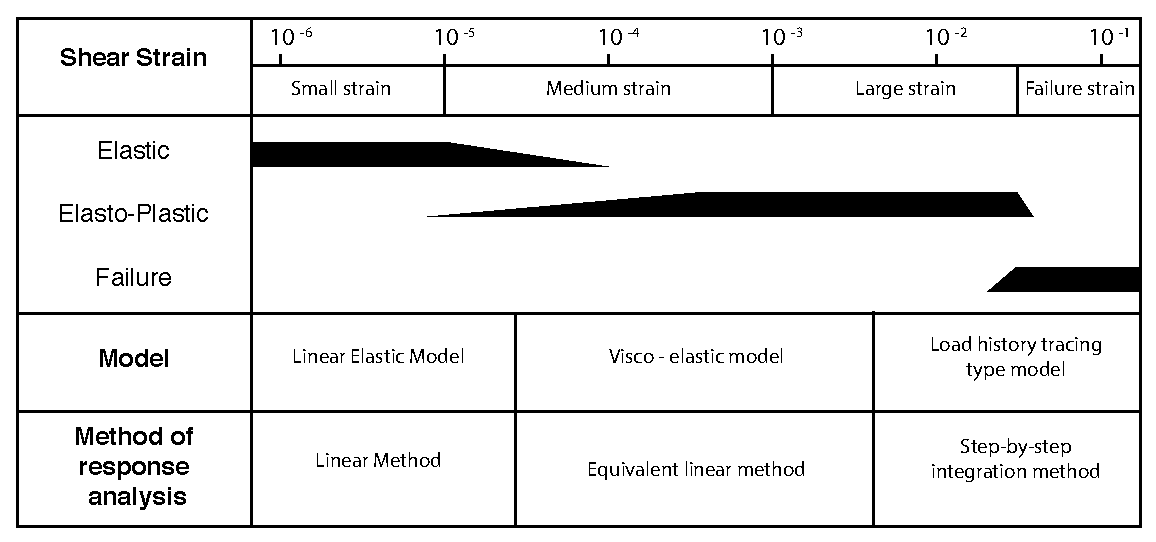
\includegraphics[width=300px]{figures/pdf/ishihara_fig_3p1.pdf}
    \caption{Modeling soil behavior based on strain level. The original figure is provided in  \citet{Ishihara_1996}}
    \label{fig:ishihara_fig_3p1}
\end{figure}



When soil behavior is expected to stay within the range of the small strain, the use of an elastic model is justified and the shear modulus is a key parameter to properly model the soil behavior. In this situation the intrinsic attenuation due to internal friction of the soil materials is considered through anelastic simulation. \citet{Assimaki2000} found the linear threshold of strain about $10^{-5}$. In cases of medium range of strains (below the level of $10^{-3}$) the soil behavior becomes elasto-plastic and the shear modulus tends to decrease with increasing shear strain, and during the cycles of load application the energy dissipation occurs. In this case the energy dissipation is mostly rate-independent and of hysteric nature, and the damping ratio can be used to represent the energy absorbing properties of soil. Due to low strain level (below the level of $10^{-3}$) the soil properties and damping level do not change with progression of load application. This kind is called non-degraded hystersis type. Linear viscoelastic models can be used to represent the soil characteristics in this strain level. For the strain level larger than about $10^{-2}$, soil properties tend to change appreciably not only with shear strain by also with the progression of cycles. This behavior is called degraded-hysteresis type. Representing the characteristics of soil behavior in this strain level needs establishing a constitutive law in which stress-strain relations can be specified at each step of loading, unloading, and reloading phases. 

Also in many other studies for 1D programs equivalent linear method and nonlinear method are used to compare the results and give an estimation about the strain boundaries that equivalent linear method remains accurate.

 \citet{Kaklamanos2015} performed a comprehensive linear, equivalent linear, and nonlinear site response analyses on 191 ground motions record at six validation site in the Kiban-Kyoshin network (KiK-net) of vertical seismometers arrays in Japan. They used linear, Equivalent linear and, fully nonlinear methods. They find that at peak shear strains from 0.01\% to 0.1\% linear site response models fail to accurately predict short-period ground motion; equivalent linear and nonlinear models offer a significant improvement at strains beyond this level, with nonlinear models exhibiting a slight improvement over equivalent-linear models at strains greater than approximately 0.05 \%. They also realized that the performance of the equivalent linear model is heavily dependent on the assumed modulus-reduction and damping relationships. 

\citet{Kim2013site} analyzed nine stations record during the 11 March 2011, Mw = 9.0 Tohoku-Oki earthquake to study the effect of long duration earthquake on site response analysis. They used 16 earthquakes and the one dimensional analysis code, DEEPSOIL. The response spectra captured by equivalent linear (ELA) and nonlinear (NL) approaches are similar for smaller earthquakes because of smaller maximum strain. For stations with maximum strain larger than 0.3\% the difference between ELA and nonlinear site response analysis is significant. 

\citet{Kaklamanos2013critical} used Kiban-Kyoshin network (Kik-net) downhole array data in Japan to analyze the accuracy (bias) and variability (precision) resulting from common site response modeling assumptions. They preformed linear and equivalent linear site response analysis at 100 KiK-net site using 3720 ground motion ranging from weak to strong. They found that the max shear strain in the soil profile, the observed peak ground acceleration at the ground surface, and the predominant spectral period of the surface ground motion are the best predictions of where evaluated models become inaccurate and/or imprecise. Linear analysis become inaccurate in predicting spectral acceleration between 0.01\% and 0.1\% shear strain for periods less than 0.5s ($f  > 2 Hz$). At spectral periods of $(T > 0.5 s)$ there is no noticeable nonlinear soil behavior. They concluded that when $\gamma_{max} > 4 \%$ the equivalent linear formulation generally under predicts ground motions for $T < 0.5 s$. For large ground motions (particularly for shear strain > 0.4 \%) SHAKE over predicts the amount of nonlinearity that actually occurs particularly at high-frequencies. 

\citet{Carlton2016comparison} compared the results of ELA and NLA. They found that in $\gamma_{max}$ greater than 0.04\% to 1.0\% there are non-negligible differences between ELA and NLA. They developed some criteria to estimate the $\gamma_{max}$ ELA before conducting the site response analysis. To do that they used 189 ground motions, nine hypothetical sites and seven actual sites. They found that for $\gamma_{max}$ ELA <0.003\% the soil behaves linearly so the difference between ELA and NLA is negligible. They found that the trend for  $\gamma_{max}ELA > 0.003\%$ is due to two opposite effects. ELA over damp ground motions for shear strain less than the effective shear strain, which reduces the total energy in the ground motion. However, for shear strains larger than the effective shear strain, ELA use smaller damping than NLA, which allows more energy to propagate to the ground surface. They found that ELA tend to predict more peaked response spectra than NLA, with longer amplification near the natural site period. They found the for period longer than 2 sec there is little difference at long periods because long period seismic waves are not as affected as short period seismic waves by shallow soft soil layers that usually experience the greatest nonlinear effects. These results are similar to \citet{Kaklamanos2013,Kim2013site} who found negligible nonlinear effects for period longer than 0.5s and 1s, respectively. They found that the best predictor of difference of ELA and NLA is the maximum shear strain induced in the soil column in ELA.

\citet{Yee2013elastic} presented a procedure to more realistically represent the large strain portion of backbone curves by asymptotically approaching the shear strength at large strains, which removes strain localization for this application and provides reasonable matches of observed and computed ground motions. They used main shock and after shock surface to rock transfer function to study the resonant frequency shift. They used ground response analyses to predict one-dimensional shear wave propagation through the soil column. They used EQL and Nonlinear method. They performed both methods in DEEPSOIL. For NL they used hyperbolic backbone curve. They proposed to adjust the soil backbone curve to transition toward a specific shear strength at large strains while preserving the small strain behavior from modulus reduction curves. They increased the small-strain material damping from laboratory-based values (near $D_{min}=1\%$) to higher level of $D_{min}=2\% and 5\%$ largely solve the problem of over prediction of high frequency ground response. They adjusted the shear strength degradation. Adjusted back bone curve could capture the shear strength at larger strains and improve the results.\\

